
\subsection{\sfind}
\label{sc-find}

Manually finding scale-dependent loops is not trivial.  Such loops can
span across multiple functions and iterate on different scale-dependent data
structures.  In Figure \ref{fig-code}, The \oonnn loops span 1000+ LOC
across 3 classes and 10 functions.
%
This difficulty motivates \sfind, a generic program analysis that helps
developers pinpoint scale-dependent loops.  The following subsections
discuss the three main steps in \sfind.







\begin{figure}[t]

\centerline{
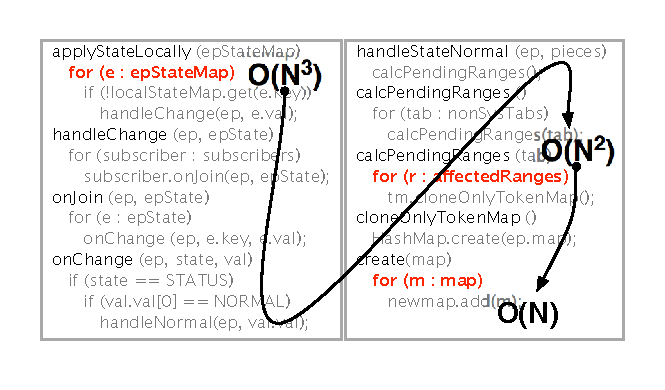
\includegraphics[height=1.7in]{F/ill/code1.eps}
%\includegraphics[height=0.6in]{F/empty.eps}
}
\vminten
\mycaption{fig-code}{\oonnn scale-depended loops}{The partial
code segment above details the \oonnn loop
in Figure \ref{fig-mot}.
Note that not all loops are scale-dependent loops.
The \ts{epStateMap}, \ts{affectedRanges}, and \ts{map}
variables are not the annotated scale-dependent variables, 
however \sfind taints them with a dataflow analysis.
}
\vminfive
\end{figure}



% $O(n^3)$ loop spans 6 functions with 188 LOC in between each pair of loops.


% ------------------------
\vni {\bf (1) Annotating scale-dependent data structures:} To use \sfind,
developers first lightly annotate scale-dependent data structures (whose
size increase as the cluster size grows).
%
For example, related to \caone (Figure \ref{fig-code}), we annotate seven
data structures and \sfind automatically taints other variables that point
to the same structures (\eg, \ts{epStateMap}, \ts{affectedRanges}, and
\ts{map} in Figure \ref{fig-code} are pointers to the annotated data
structures).


%(\ts{endpointStateMap}, \ts{tokenToEndpointMap},
%\ts{endpointToHostIdMap}, and \ts{bootstrapTokens});



% ------------------------
\vni {\bf (2) Finding scale-dependent loops:}
%
With the annotations, \sfind can then automatically find scale-dependent
loops with the following steps:
%
(a) perform a data-flow analysis to taint other pointers derived from the
original scale-dependent variables,
%
(b) taint loops (\ts{for}, \ts{while}) that iterate through the variables,
%
(c) perform a control-flow analysis to construct the nested Big $O$
complexity of each loop,
%
(d) identify the nested-loop contents (CPU/instructions only, IOs, or
locks).
%
With these steps, in Figure \ref{fig-code} for example, \sfind can mark
\ts{applyStateLocally} as an \oonnn function.


We also notice a special case of 
scale-dependent ``loops'': 
In master-worker architecture, a synchronized master's function
that is being called by all the worker nodes implicitly forms a ``loop''
(examples in \sec\ref{eval-bugs}).  
%
\sfind also handles such a scenario; the developers simply annotate the
master RPC class and \sfind automatically searches for locking
functions called by the worker nodes.  \sfind also differentiates
functions that are called within the client read/write paths (higher call
frequency) and by background periodic threads.

% if have space:
%
% Developers can prioritize those within the
% client paths, as they run most of the time.
%
% Due to space constraints, we omit discussion of other challenges such as
% abstract classes, \xxx

% ------------------------
\vni {\bf (3) Reporting and triaging:}
%
Before producing a report, \sfind performs a simple triaging.  For
example, if a function $g$ has a lower complexity than $f$ and $g$ is
within the call path of $f$, then developers can prioritize testing $f$.
%
For every nested loop to test, \sfind reports the relevant control- and
data-flows from the outer-most to inner-most loop, along with the entry
points (either client/admin RPCs or background daemon threads).
%
This helps developers create the necessary test workloads.  For example,
in Figure \ref{fig-code}, the \oonnn path is only exercised if the cluster
bootstraps from scratch; peers do not know about each other (hinted from
the \ts{if(!localStateMap.get())}, \ts{onChange()}, \ts{state==STATUS} and
\ts{val==NORMAL}).

% creating the unit tests
We note that creating test workloads from \sfind's reports is a manual
process.  Automated test generation is possible for single-machine
programs/libraries \cite{Cadar+08-KLEE}, however we are not aware of any
work that automates such process in the context of real-world, complex,
large-scale distributed systems.
%
We put our work in the context of DevOps culture
\cite{Limoncelli+11-Devops} where developers are testers and testers are
developers, which simplify testing efforts.



\if 0
With this triaging, we reduce the
number of tests.  For example, in Cassandra, out of 22 \oonn and 9 \oonnn
functions, they are accessible by 3 \oonnn functions.
\fi


% the content of the loop
% (CPU, lock, IO) along with the total number of LOC inside the loop, which
% can help developers to prioritize.

